
\begin{frame}
    \frametitle{Системы координат}
    \begin{itemize}
        \item Локальные системы координат
        \item Географические системы координат
        \item Спроецированные (прямоугольные) системы координат
    \end{itemize}
\end{frame}

\begin{frame}
    \frametitle{Как различать по значениям координат}
    \begin{itemize}
        \item Локальные системы координат: от 0,0 до, например, 5000,6000
        \item Географические системы координат: от -180,-90, до 180,90
        \item Спроецированные (прямоугольные) системы координат: от -1000000,1000000 до, например, 1000000, 1000000
    \end{itemize}
\end{frame}


\begin{frame}
    \frametitle{Локальные системы координат}
    \begin{figure}[!ht]
        \begin{center}
            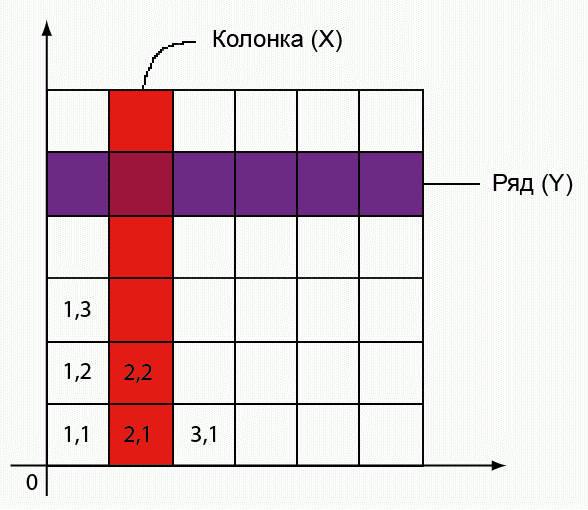
\includegraphics[width=0.6\columnwidth]{./coordinates/img/local_coord}
        \end{center}
    \end{figure}
\end{frame}

\begin{frame}
    \frametitle{Географические координаты}
    \begin{figure}[!ht]
        \begin{center}
            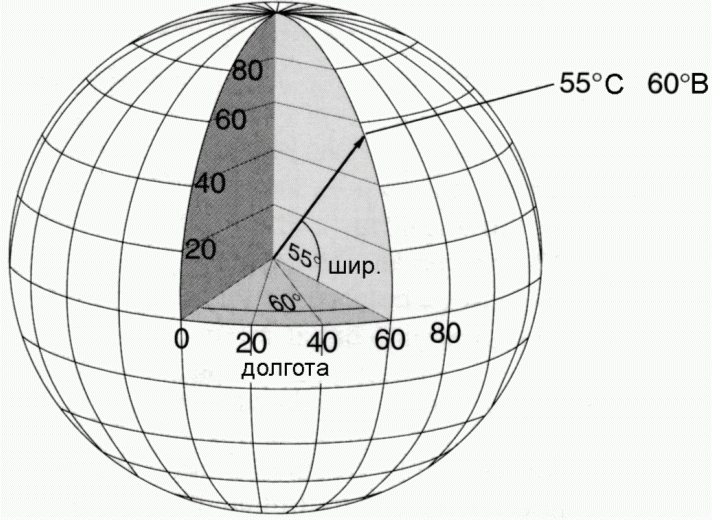
\includegraphics[width=0.6\columnwidth]{./coordinates/img/geo_coord}
        \end{center}
    \end{figure}

    Широта --- угол между  плоскостью экватора и нормалью к поверхности эллипсоида в данной точке (0-90 с.ш. и ю.ш.)

    Долгота --- угол между меридианом данной точки и начальным меридианом (0-180 з.д. и в.д.)
\end{frame}



\begin{frame}
    \frametitle{Геоид}
    \begin{figure}[!ht]
        \begin{center}
            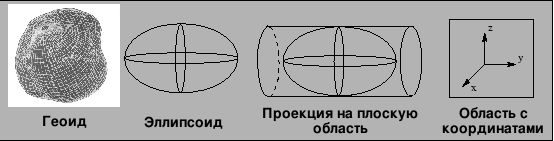
\includegraphics[width=0.7\columnwidth]{./coordinates/img/geoid.png}
        \end{center}
        \caption{Понятие геоида, элипсоида и проекции}
    \end{figure}
    \begin{description}
        \item[Геоид] Форму Земли, особенно с учетом рельефа, можно описать с помощью геоида. Эта фигура является результатом сложных физических расчётов гравитационного поля Земли. Из-за неоднородного распределения массы поле оказывается разным в разных регионах, что приводит к деформации сферы. Таким образом, геоид представляет гравитационое поле Земли.
    \end{description}
    Ввиду математической сложности геоида, в качестве приближения формы Земли в географических информационных системах используется сфера или эллипсоид.
\end{frame}

\begin{frame}
    \frametitle{Эллипсоид}
    \begin{figure}[!ht]
        \begin{center}
            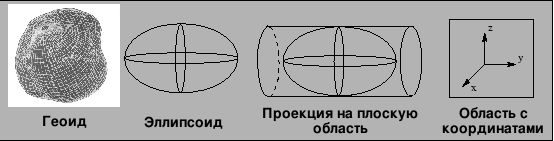
\includegraphics[width=0.8\columnwidth]{./coordinates/img/geoid.png}
        \end{center}
        \caption{Понятие геоида, элипсоида и проекции}
    \end{figure}

    Упрощённое представление формы Земли сферой недостачно точно для создания карт масштаба крупнее 1:2~000~000. Эллипсоиды вращения или сфероиды пытаются воспроизвести сложную форму Земли насколько возможно точно математически. Поэтому расстояние от полюса до центра Земли меньше, чем от экватора.

    Существует ряд моделей эллипсоидов, дающих оптимальные результаты для разных регионов. В общем, для каждого региона можно подобрать эллипсоид, являющийся достаточно точным приближением поверхности Земли в этом регионе.

\end{frame}

\begin{frame}
    \frametitle{Примеры референц-эллипсоидов}
    \begin{table}[h]
    \centering
    \begin{tabular}[c]{p{0.2\linewidth}|p{0.15\linewidth}|p{0.15\linewidth}|p{0.3\linewidth}}
    {Эллипсоид, представ\-ляющий Землю} & Большая полуось (м) & Малая полуось (м) & Область применения\\[2mm]\hline
     WGS 1984 & 6378137 & 6378137 & Северная Америка, весь мир\\
     Эллипсоид Крассовского & 6378245 &6356863 & Российская Федерация, страны бывшего CCCР\\
     & & &
    \end{tabular}\caption{Примеры распространенных эллипсоидов}
    \end{table}
\end{frame}

\begin{frame}
    \frametitle{Датум}
    {\tiny Эллипсоид задаёт абстрактную модель конфигурации земной поверхности. Для того, чтобы можно было отсчитывать координаты точки на поверхности эллипсоида --- нужны оси координат.}

    \begin{description}
        \item[Датум:] набор параметров смещения и поворота референц-эллипсоида для лучшей апроксимации земной поверхности. Также датум задаёт нулевой меридиан, от которого будет идти отсчёт долготы.
    \end{description}
    { \small
   Датумы бывают
   \begin{itemize}
       \item глобальными, т.е. предназначенными для аппроксимации земной поверхности на территории всей планеты. Например, датум WGS84 базирующийся на собственном эллипсоиде.
       \item локальными, т.е. предназначенными для лучшей аппроксимации участка земной поверхности. Пример: <<Пулково 1942>> --- датум, основывающийся на эллипсоиде Крассовского, и предназначенный для лучшей аппроксимации территории Советского Союза.
    \end{itemize}
    }
   {\tiny На базе одного референц-эллипсоида может основываться несколько различных датумов. Так, многие страны восточной Европы имели собственные датумы, основанные на эллипсоиде Крассовского.}
\end{frame}


\begin{frame}
    \frametitle{Переход от одного датума к другому}
    \begin{figure}[!ht]
        \begin{center}
            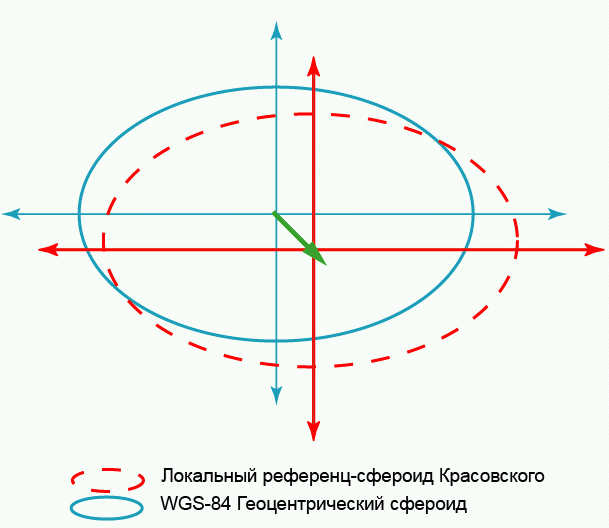
\includegraphics[width=0.6\columnwidth]{./coordinates/img/coord_transition}
        \end{center}
    \end{figure}
\end{frame}


\begin{frame}
    \frametitle{Три семейства картографических проекций\footnote{Материал раздела опирается на "Краткое введение в ГИС" \url{http://gis-lab.info/qa/gentle-intro-gis.html}}}
    \begin{figure}[!ht]
        \begin{center}
            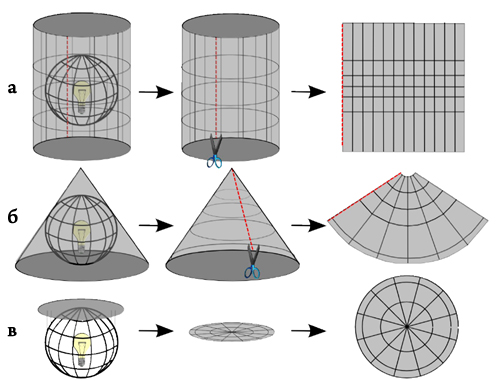
\includegraphics[width=0.75\columnwidth]{./coordinates/img/proj_fam.jpg}
        \end{center}
        \caption{а) цилиндрические, б) конические и в) плоскостные (азимутальные) проекции}
    \end{figure}
\end{frame}

\begin{frame}
    \frametitle{Виды искажений}
    В ходе проецирования любая карта будет иметь искажения
    \begin{itemize}
        \item углов,
        \item расстояний,
        \item площадей.
    \end{itemize}
    возможны искажения одновременно нескольких параметров.

    Поэтому важно подобрать проекцию карты под решаемую задачу.

\end{frame}

\begin{frame}
    %\frametitle{Конформные проекции}
    \begin{description}
        \item[Равноугольная (конформная) проекция:] картографическая проекция, позволяющая передавать на картах углы без искажений и сохранять в каждой точке постоянный масштаб по всем направлениям, хотя в разных местах карты масштаб различен.
    \end{description}
    Используются для навигационных, метеорологических и др. задач, где важно сохранение углов.
    \begin{figure}[!ht]
        \begin{center}
            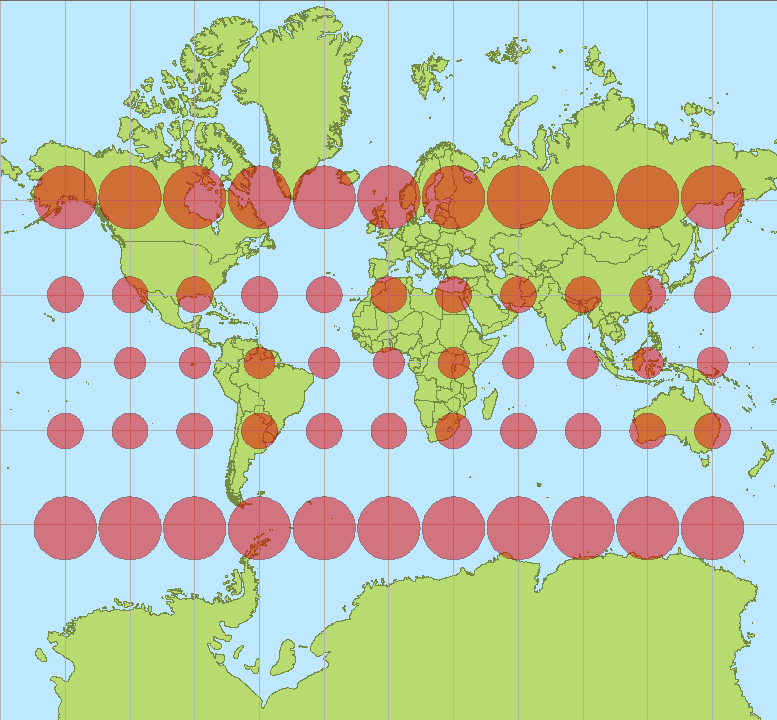
\includegraphics[width=0.5\columnwidth]{./coordinates/img/merkator.png}
        \end{center}
        \caption{Пример --- проекция Меркатора.}
    \end{figure}

\end{frame}

\begin{frame}
    %\frametitle{Равнопромежуточные проекции}
    \begin{description}
        \item[Равнопромежуточная проекция:] картографическая проекция, обладающая свойством сохранения масштаба вдоль определенных линий.
    \end{description}
    Равнопромежуточные проекции обеспечивают правильные расстояния от центра проекции вдоль определенных линий. Эти проекции используются для сейсмического картографирования, а также для задач навигации.
    \begin{figure}[!ht]
        \begin{center}
            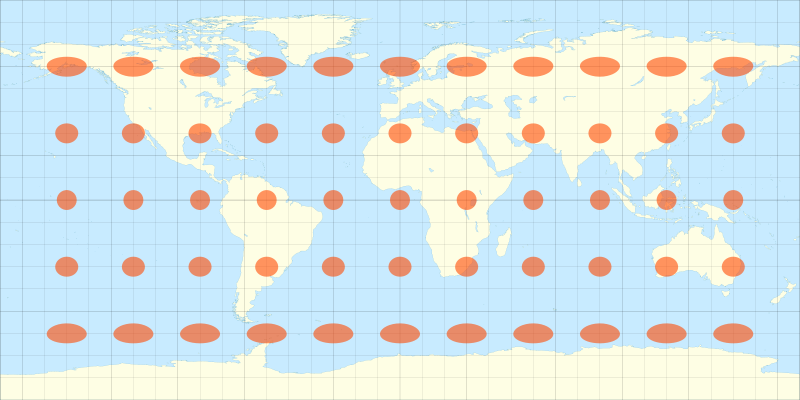
\includegraphics[width=0.8\columnwidth]{./coordinates/img/equidistant.png}
        \end{center}
        \caption{Пример --- простая цилиндрическая проекция (plate carrée)}
    \end{figure}
\end{frame}

\begin{frame}
    %\frametitle{Равновеликие проекции}
    \begin{description}
        \item[Равновеликая проекция:] картографическая проекция, которая не искажает площадей и сохраняет на всей карте единый масштаб площадей
    Площади фигур на карте пропорциональны площадям соответствующих фигур в реальности, но при этом сильны искажения углов и форм.
    \end{description}
    \begin{figure}[!ht]
        \begin{center}
            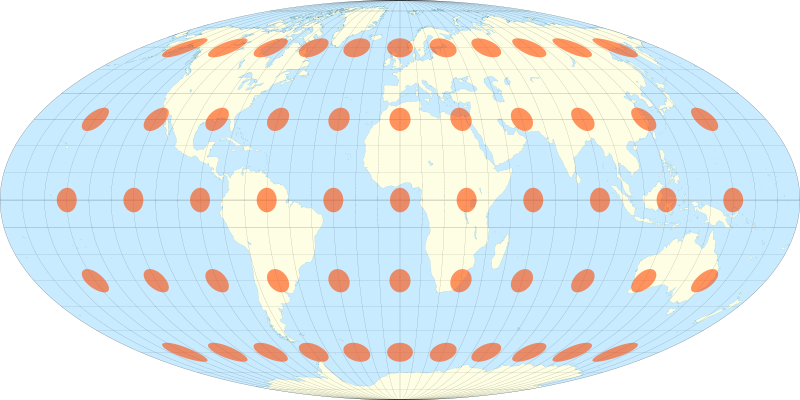
\includegraphics[width=0.85\columnwidth]{./coordinates/img/mollweide.png}
        \end{center}
        \caption{Пример --- равновеликая цилиндрическая проекция Мольвейде }
    \end{figure}

\end{frame}


\begin{frame}
    \frametitle{Системы координат}
    После того, как поверхность земного шара или её часть спроецирована на плоскость, следует задать систему координат, чтобы точно размещать 2-~или 3-мерные участки на карте.

    С помощью систем координат каждое место на Земле может быть описано набором из трех цифр, называемых координатами. Системы координат делят на
    \begin{itemize}
        \item системы географических координат;
        \item системы проекционных координат (также называются картезианскими, или прямоугольными).
    \end{itemize}
\end{frame}

\begin{frame}
    \frametitle{Географические системы координат}

    Географическая система (Longitude-Latitude, lon/lat): Наиболее часто используемая система, использующая долготу, широту и высоту.

    Координаты отсчитываются от нулевого меридиана и экватора. В результате, поверхность земли покрывает сетка из 180 меридианов (долгот) на запад и восток от Гринвича и 180 параллелей (широт) на север и юг от экватора.

    Высота измеряется от центра Земли.

    Единицы системы могут быть выражены в шестидесятеричном (градусы:минуты:секунды, буква, обозначающая направление) или десятичном (+/- градусы с десятичными знаками) исчислении.
\end{frame}


\begin{frame}
    \frametitle{Системы проекционных координат}
    Будут рассмотрены две распространенные системы:
    \begin{itemize}
        \item Система координат (проекция) Гаусса-Крюгера;
        \item Система координат (проекция) UTM (Universal Transverse Mercator)
    \end{itemize}

\end{frame}

\begin{frame}
    \frametitle{Система кординат Гаусса-Крюгера}
    \begin{figure}[!ht]
        \begin{center}
            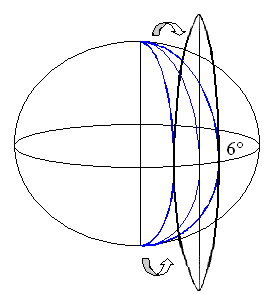
\includegraphics[width=0.4\columnwidth]{./coordinates/img/gauss_kruger1.png}
        \end{center}
        \caption{Схема построения 6-градусных зон}
    \end{figure}
    Вся поверхность Земли делится на 6-градусные (по долготе) зоны (дольки от полюса до полюса), которые каждая отдельно разворачиваются в плоскую поверхность. Всего образуется 60 таких зон, которые нумеруются цифрами от 1 до 60.

\end{frame}

\begin{frame}
    \frametitle{Зоны}
    \begin{figure}[!ht]
        \begin{center}
            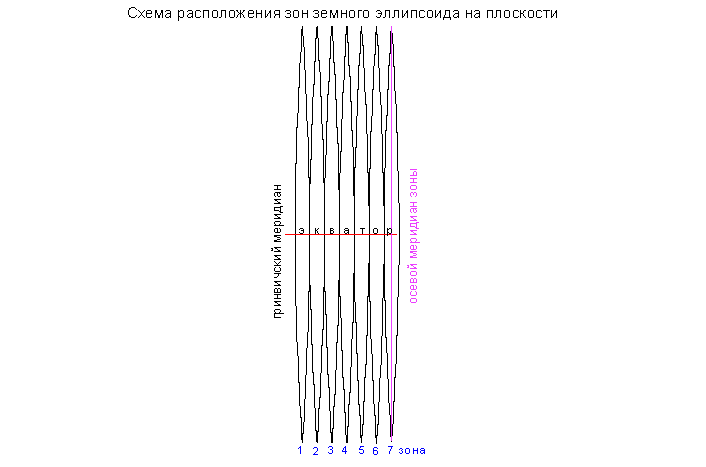
\includegraphics[width=0.6\columnwidth]{./coordinates/img/zonesgk_l.png}
        \end{center}
    \end{figure}
     Зоны нумеруются с запада на восток, начиная с 0: зона 1 простирается с меридиана 0 до меридиана 6, её центральный меридиан 3. Зона 2 --- с 6 до 12, и т.д.

     Цилиндр разворачивают в плоскость и накладывают прямоугольную километровую сетку. За ось OX принимают изображение осевого меридиана зоны (положительное направление --- на север), за ось OY принимают изображение экватора (положительное направление --- на восток).
\end{frame}

\begin{frame}
    \frametitle{Координаты внутри зоны}
    \begin{figure}[!ht]
        \begin{center}
            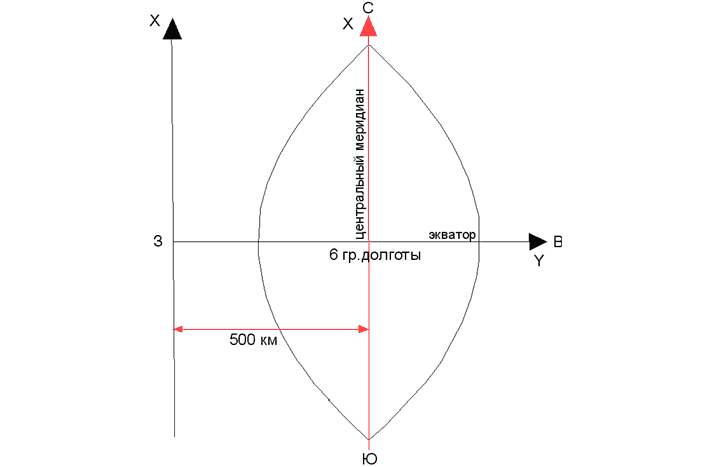
\includegraphics[width=0.35\columnwidth]{./coordinates/img/gauss_kruger2.png}
        \end{center}
    \end{figure}
    В каждой из шестиградусных зон своя система прямоугольных координат. Вертикальные линии сетки параллельны центральному меридиану. Для того, чтобы все прямоугольные координаты были положительны, вводится восточное смещение (false easting), равное 500~000 м, т.е. координата Y на центральном меридиане равна 500~000 м. Для определенности, чтобы только по численному значению координаты Y можно было определить, к какой зоне относятся эти значения, к ним слева приписывается номер зоны.

    Пример: (X=6~177~200; Y=7~420~000) --- 7 зона, на 80 км западнее среднего меридиана зоны 7, на 6~177~200 метров севернее экватора.

\end{frame}

\begin{frame}
    \frametitle{UTM}
    Система координат UTM по построению похожа на систему Гаусса-Крюгера:
    \begin{itemize}
        \item делит Землю на 60 вытянутых в меридиональном направлении зон шириной 6 градусов;
        \item отображающая их по отдельности в равноугольной поперечно-цилиндрической проекции Меркатора.
    \end{itemize}

     Отличия:
     \begin{itemize}
         \item используется масштабный коэффициент, равный 0,9996.% Поэтому эта система координат сохраняет масштабы не на осевом меридиане, а на некотором расстоянии (около 180 км) от него, из-за чего максимальное искажение масштаба в пределах шестиградусной зоны у неё меньше.
         \item нумерация зон: первая зона та, осевой меридиан которой имеет долготу 177 з.д. % Таким образом, например, 7-я зона в системе координат Гаусса—Крюгера по географическому охвату соответствует 37-й зоне UTM.
         \item Ось абсцисс в данной системе координат направлена на восток, а ось ординат --- на север. Во избежание отрицательных значений координат, к значению абсциссы прибавляются 500~000~м, а к значению ординаты в южном полушарии --- 10~000~000~м
     \end{itemize}
\end{frame}

\begin{frame}
    \frametitle{Важно помнить}
    \begin{itemize}
        \item Всегда уточняйте в какой системе координат данные
        \item Убедитесь, что у слоев всегда есть файл описания проекции *.prj
        \item Если это таблица с координатами, уточняйте в каком они формате
    \end{itemize}
\end{frame}



\begin{frame}
    \frametitle{Литература}
    \begin{enumerate}
        \item \url{http://gis-lab.info/docs/grass/tutorial60/04r.html}
        \item \url{http://gis-lab.info/qa/gentle-intro-gis.html}
        \item \url{http://giscraft.ru/info/cs/cs.shtml}
    \end{enumerate}
\end{frame}




